\section{Versuchsreihe}
\label{section:verkehr/versuchsreihe}

Um zwei der vorgestellten Suchalgorithmen zu vergleichen, wurden zwei Versuchsreihen erstellt. Dazu wurden in einem ersten Schritt zufällige Netzwerke generiert und anschliessend der \emph{Dijkstra}-, sowie der \emph{$A^*$}-Algorithmus auf das Netzwerk angewandt.
Dieser Vorgang wurde für die zufällig generierten Netzwerke mit einer Knotenzahl von 10, 20 50, 100, 200, 500 und 1000 je zehnmal repetiert.
Die Anzahl der Knoten im abgesuchten Netzwerk wirkt sich direkt auf die Rechenzeit aus. Der \emph{Dijkstra}-Algorithmus weist eine Zeitkomplexität von $\mathcal{O}(E\log{}V)$ auf, wobei $E$ die Anzahl Kanten (engl. \emph{edges}) und $V$ die Anzahl Knoten (engl. \emph{vertices}) darstellt.
Für den \emph{A*}-Algorithmus ist die Zeitkomplexität einerseits abhängig von der verwendeten Heuristik, andererseits aber auch vom vorliegenden Netzwerk selbst. Aus diesem Grund lässt sich keine defintive Angabe zu $\mathcal{O}$ machen.

Die beiden Versuchsreihen unterscheiden sich zudem dahingehend, dass der Start- und Zielknoten bei der ersten Versuchsreihe im Netzwerk diametral gegenüber liegen. Dadurch gehen viele Knoten verloren, welcher \emph{Dijkstra} als uninformierter Suchalgorithmus absuchen würde. In der zweiten Veruschsreihe werden hingegen Start- un Zielpunkt zufällig im Netzwerk ausgewählt. Es wird deshalb erwwartet, dass die Unterschiede in der Rechenzeit der beiden Algorithmen in der zweiten Versuchsreihe deutlich ausgeprägter sind.

\subsection{Einfluss der Knotenzahl auf die Rechenzeit}
\label{verkehr:Knotenzahl}

\begin{figure}
\centering
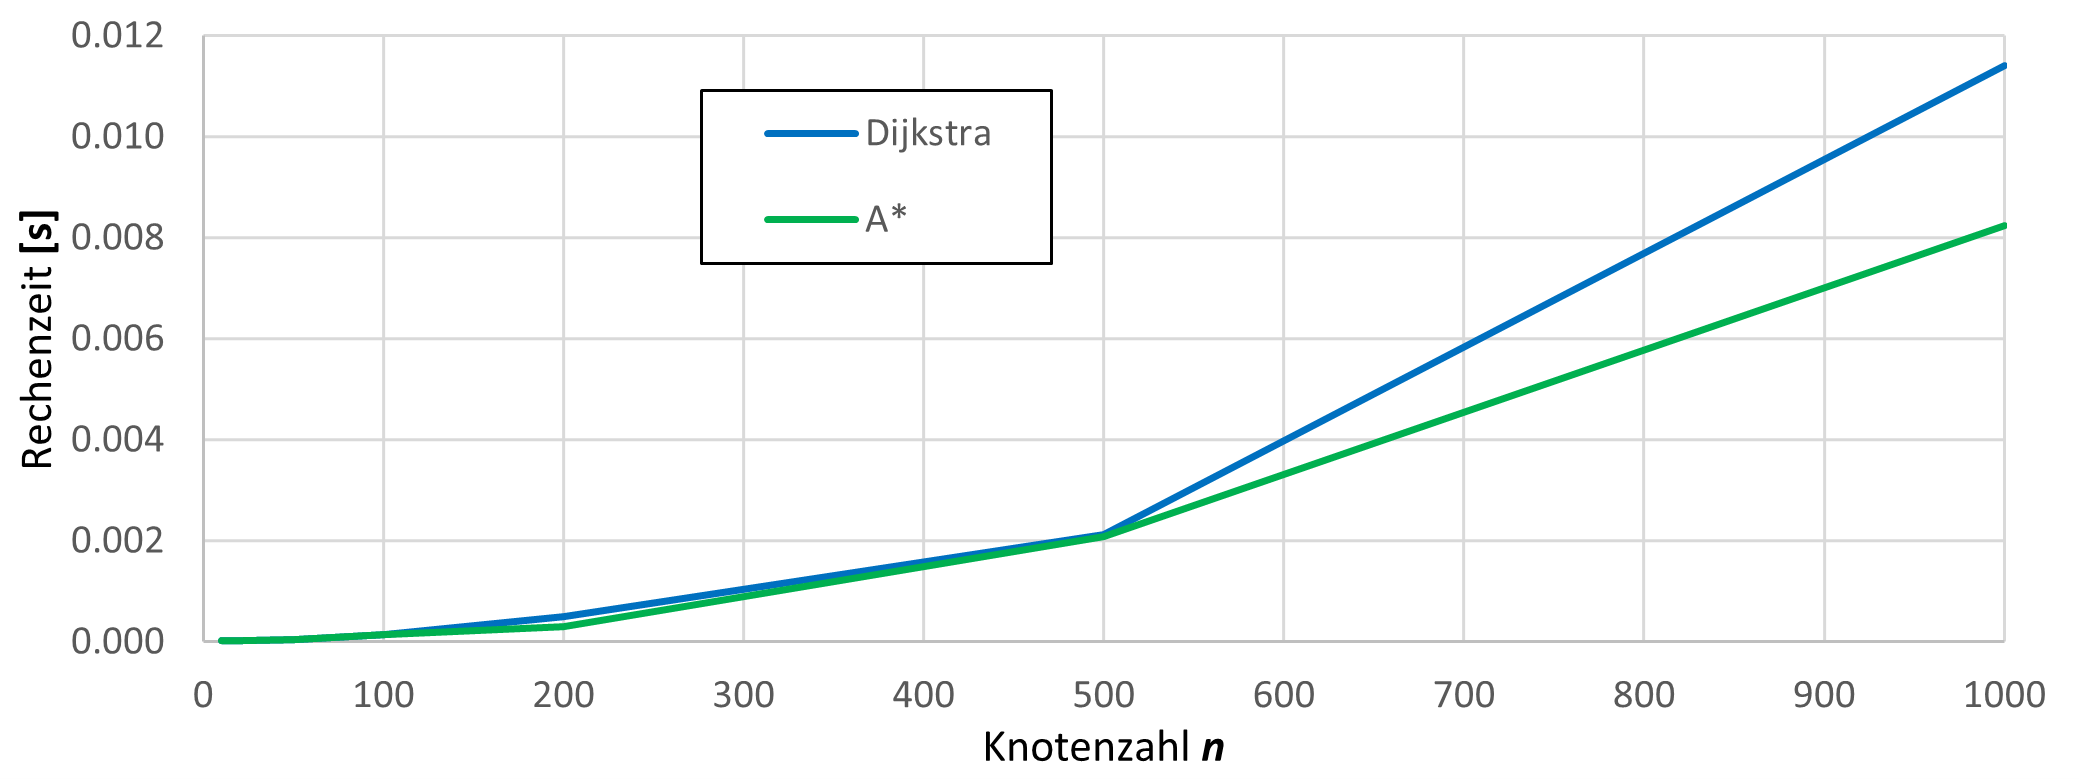
\includegraphics[width=12cm]{papers/verkehr/figures/chart_Vr1.png}

\caption{Gemessene Rechenzeiten der ersten Versuchsreihe in Abhängigkeit der Knotenzahl.}
\label{verkehr:Vr1}
\end{figure}

In \ref{verkehr:Vr1} ist ersichtlich, dass der Unterschied in der Rechenzeit zwischen \emph{Dijkstra} und \emph{A*} erst aber einer Knotenzahl von ca. $n=500$ merklich ansteigt. Dieses etwas überraschende Resultat ist darauf zurückzuführen, dass bei steigender Knotenzahl die Abweichung des effektiven kürzesten Pfades von der Distanz der Luftlinie abnimmt.
Die Effektivität von \emph{A*} mit euklidischer Heuristik ist wiederum grösser, wenn die Abweichung des kürzesten Pfads von der Luftlinie minimal ist.
Bei Betrachtung von \ref{verkehr:pathDifference} wird dies ersichtlich, wobei die relative Abweichung erstaunlicherweise bei einer Knotenzahl von $n=100$ maximal ist und nach $n=500$ nur noch marginal abnimmt.

\begin{figure}
\centering
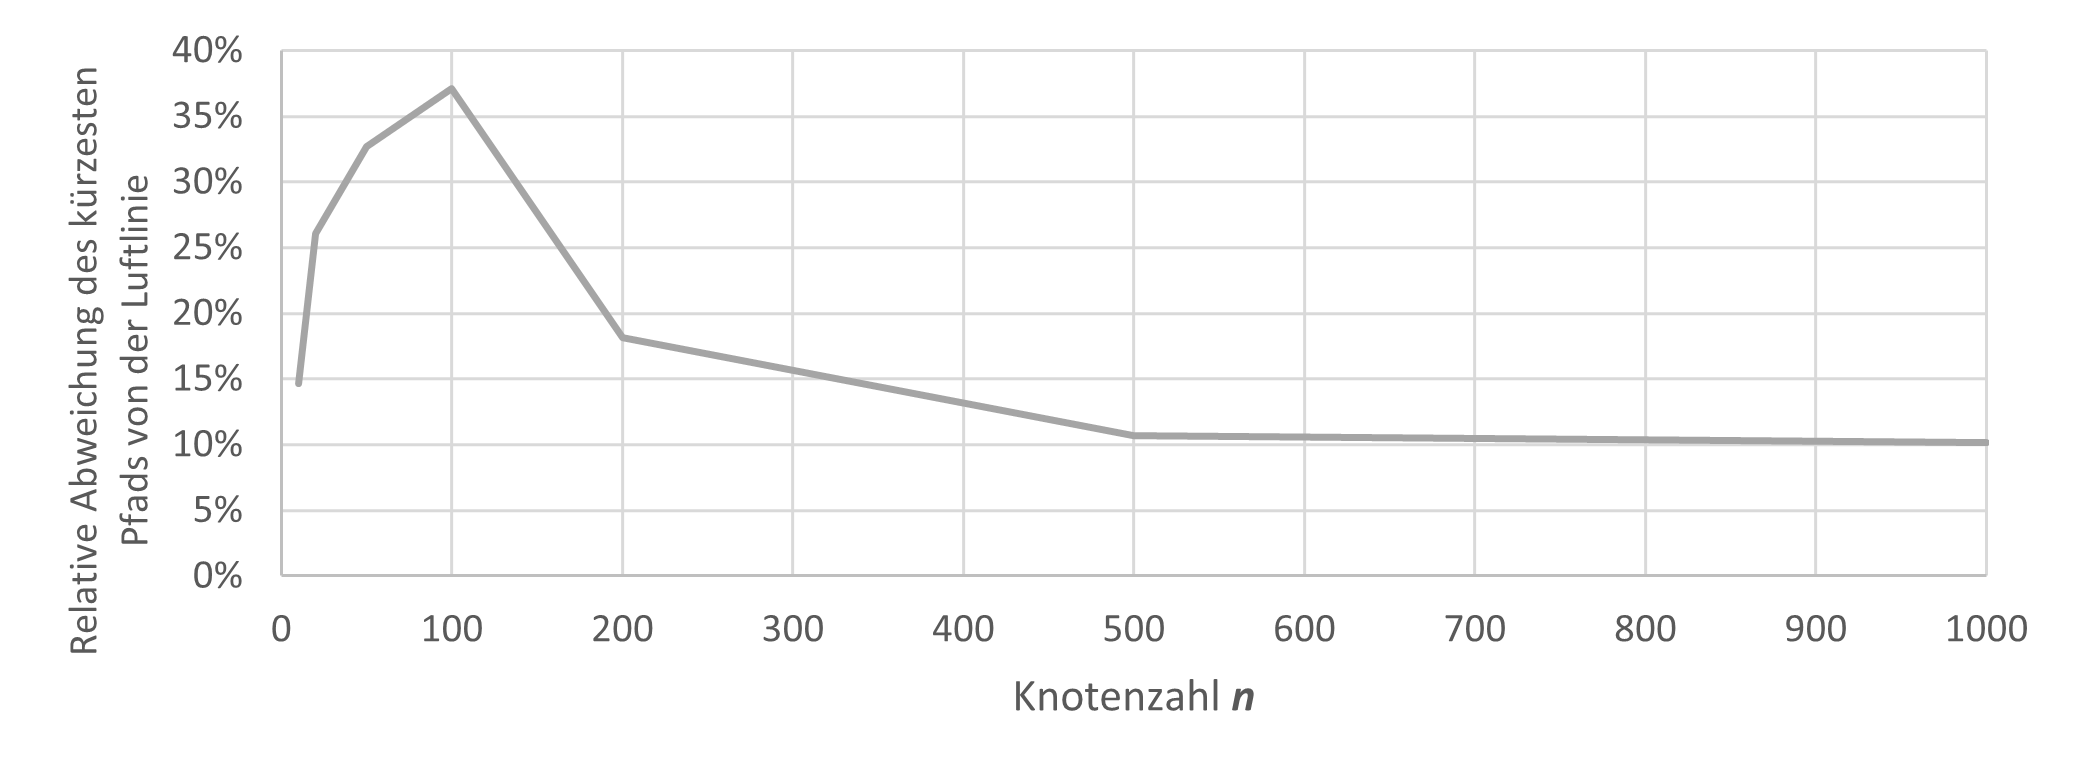
\includegraphics[width=12cm]{papers/verkehr/figures/chart_pathDiff.png}

\caption{Relative Abweichung des kürzesten Pfads von der Luftlinie.}
\label{verkehr:pathDifference}
\end{figure}


\subsection{Einfluss der Position der Start- und Zielknoten auf die Rechenzeit}

\begin{figure}
\centering
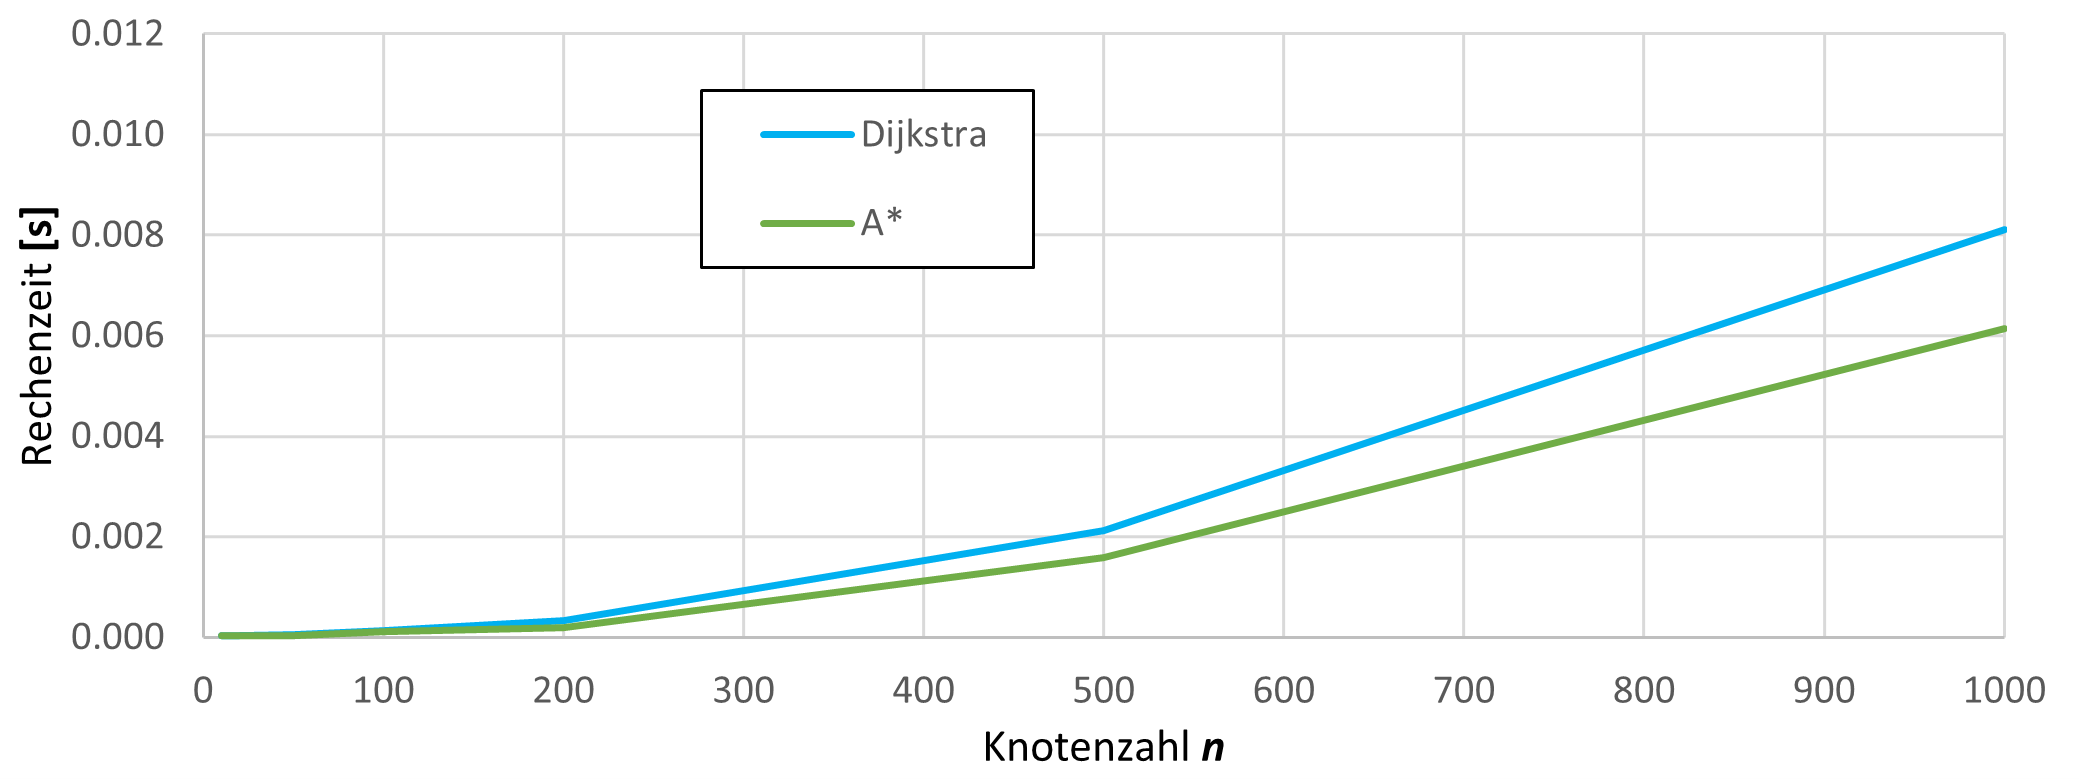
\includegraphics[width=12cm]{papers/verkehr/figures/chart_Vr2.png}\\
\caption{Gemessene Rechenzeiten der zweiten Versuchsreihe in Abhängigkeit der Knotenzahl.}
\label{verkehr:Vr2}
\end{figure}

Zum Vergleich der Resultate in \ref{verkehr:Knotenzahl} zeigt \ref{verkehr:Vr2} die Rechenzeiten der zweiten Versuchsreihe, in welcher die Start- und Zielknoten zufällig im Netzwerk ausgewählt wurden. Einerseits ist eine reduzierte durchschnittliche Rechenzeit festzustellen, was schlicht daran liegt, dass die zufällige Wahl der Knoten dazu führt, dass diese tendenziell weniger weit auseinander liegen.\\
Des weiteren ist festzustellen, dass sich die Unterschiede der Rechenzeiten zwischen  \emph{Dijkstra} und \emph{A*} deutlich früher abzeichnen. Dieses Phänomen lässt sich leicht durch die zielgerichtete Suche des \emph{A*}-Algorithmus erklären.

\begin{figure}
\centering
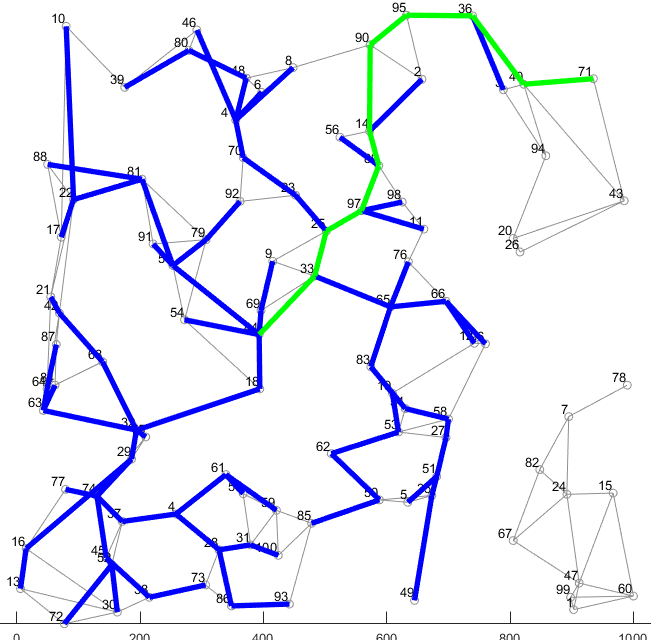
\includegraphics[width=6cm]{papers/verkehr/figures/network_dij.png}\qquad
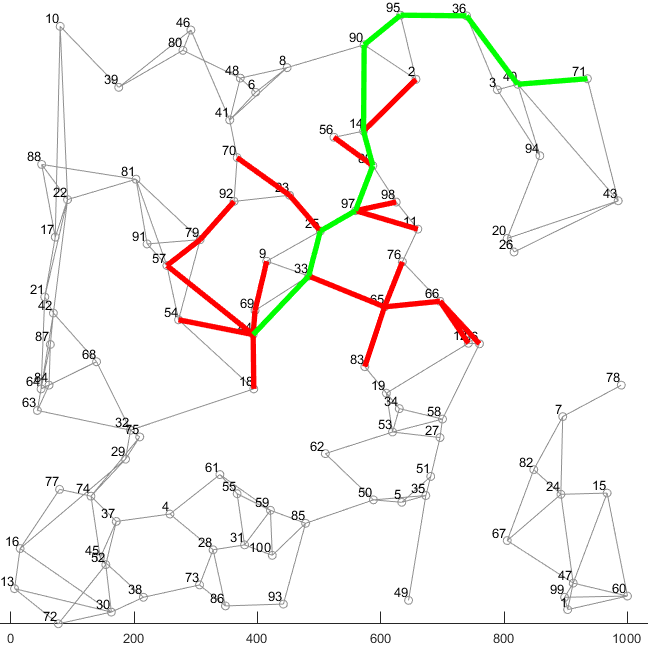
\includegraphics[width=6cm]{papers/verkehr/figures/network_aStar.png}
\caption{Suchpfad in grün mit \emph{Dijkstra} (links), und \emph{A*} (rechts). Besuchte Knoten sind in blau, resp. rot markiert.}
\label{verkehr:Comparison}
\end{figure}

In \ref{verkehr:Comparison} ist ersichtlich, dass bei einem im Netzwerk liegenden Startknoten die zielgerichtete Suche von \emph{A*} deutlich ausgeprägter zum Zuge kommt, als wenn dieser am Rand des Netzwerks liegen würde.
